
\documentclass[12pt]{article}
\usepackage[brazil]{babel}
\usepackage[utf8]{inputenc}
\usepackage{amsmath}
\usepackage{amsfonts}
\usepackage{amssymb}
\usepackage{geometry}
\usepackage{graphicx}
\usepackage{float}
\usepackage{enumitem}
\usepackage{multicol}
\usepackage{array}
\usepackage{xcolor}
\usepackage[T1]{fontenc}
\usepackage{mathptmx} %times new roman


\geometry{a4paper, margin=1.2cm}
\setlength{\parindent}{1.2cm}

% implementa contador
% Definindo o contador e o comando de questão
\newcounter{questao}
\newcommand{\novaquestao}[1]{%
	\stepcounter{questao}%
	\subsection*{Questão \thequestao\ (#1)}%
}

\begin{document}
	% Cabeçalho reduzido
	\vspace{0.5cm}
	\begin{center}
		\large
		\begin{tabular}{|l l|}
			\hline
			\textbf{ESCOLA:} & EETI GILBERTO MESTRINHO DE MEDEIROS RAPOSO \\ 
			\textbf{ALUNA(O):} & \underline{\hspace{7cm}} \textbf{SÉRIE:} \underline{\hspace{1.5cm}} \textbf{TURMA:} \underline{\hspace{1.5cm}} \\
			\textbf{PROFESSOR:} & \underline{\hspace{7cm}} \textbf{DATA:} \underline{\hspace{1.5cm}}/\underline{\hspace{1.5cm}}/\underline{\hspace{1.5cm}} \\
			\textbf{VALOR:} & \underline{\hspace{3cm}} \textbf{NOTA:} \underline{\hspace{1.5cm}} \\
			\hline
		\end{tabular}
	\end{center}
	\vspace{0.5cm}
	
	% Título manual
	\begin{center}
		\Large\textbf{AV1 - 3º BIMESTRE}
	\end{center}
	
	\vspace{0.3cm}
	
	\section*{\textbf{ATENÇÃO:}}
	\begin{itemize}[noitemsep]
		\item Resolva toda a PROVA, justificando cada questão.
		\item Colocar o nome completo e identificação no cabeçalho.
		\item Há apenas uma opção correta em cada questão de múltipla escolha.
	\end{itemize}
	% Início das colunas com linha vertical
	%\mostravermelhotrue
	\begin{multicols}{2}
		\columnseprule=0.4pt
		\columnsep=20pt
		
		\novaquestao{Enem 2020}
		
			O Estatuto do Idoso, no Brasil, prevê certos direitos às pessoas com idade avançada, concedendo a estas, entre outros benefícios, a restituição de imposto de renda antes dos demais contribuintes. A tabela informa os nomes e as idades de 12 idosos que aguardam suas restituições de imposto de renda. Considere que, entre os idosos, a restituição seja concedida em ordem decrescente de idade e que,
			em subgrupos de pessoas com a mesma idade, a ordem seja decidida por sorteio.
			
			\begin{center}
				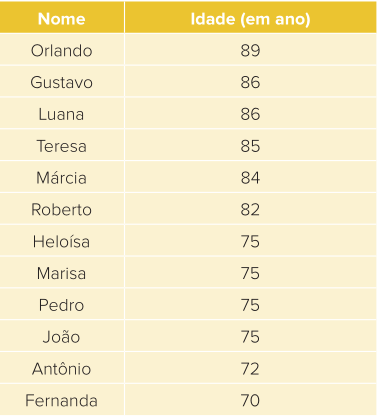
\includegraphics[scale=0.6]{imagens/enem-2020.png}
			\end{center} Nessas condições, a probabilidade de João ser a sétima pessoa do grupo a receber sua restituição é igual a:
			
			\begin{enumerate}[label=(\alph*), noitemsep]
				\item {1}/{12}
				\item {7}/{12}
				\item {1}/{8}
				\item {5}/{6}
				\item {1}/{4}
			\end{enumerate}
		
		\novaquestao{Enem PPL 2020}
		
			Para um docente estrangeiro trabalhar no Brasil, ele necessita validar o seu diploma junto ao Ministério da Educação. Num determinado ano, somente para estrangeiros que trabalharão em universidades dos estados de São Paulo e Rio de Janeiro, foram validados os diplomas de 402 docentes estrangeiros. Na 
			tabela, está representada a distribuição desses docentes estrangeiros, por países de origem, para cada um dos dois estados.
			
			\begin{center}
				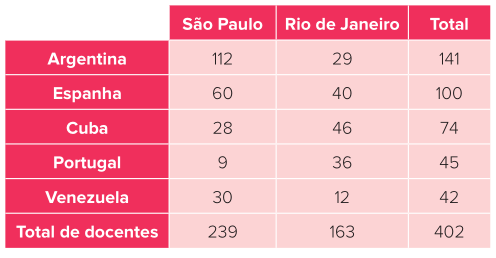
\includegraphics[scale=0.5]{imagens/enem-ppl-2020.png}
			\end{center} A probabilidade de se escolher, aleatoriamente, um docente espanhol, sabendo-se que ele trabalha em uma universidade do estado de São Paulo é:
			
			\begin{enumerate}[label=(\alph*), noitemsep]
				\item {60}/{402}
				\item {60}/{239}
				\item {60}/{100}
				\item {100}/{239}
				\item {279}/{402}
			\end{enumerate}
			
		\novaquestao{UEA SIS II 2017}
		
			Ana e Beatriz são alunas de uma classe onde foram sorteados
			dois livros para dois estudantes diferentes. Essa classe tem 10
			meninas e 12 meninos e no primeiro sorteio saiu o nome de Ana. Ao
			sortear o segundo nome, a professora avisou que era de uma menina
			e Beatriz calculou corretamente que a probabilidade de ter sido ela
			a sorteada era:
			
			\begin{enumerate}[label=(\alph*), noitemsep]
				\item {1}/{3}
				\item {1}/{5}
				\item {1}/{8}
				\item {1}/{9}  %
				\item {1}/{10}
			\end{enumerate}
			
		\novaquestao{UEA SIS II 2021}
		
			Melissa e Janaína compraram, independentemente uma da
			outra, ingressos para uma mesma sessão de cinema. Se os
			assentos que elas compraram estão na fileira G, que possui 10
			assentos lado a lado, a probabilidade de que as duas sentem-se
			uma ao lado da outra é:
			
			\begin{enumerate}[label=(\alph*), noitemsep]
				\item 5\%
				\item 10\%
				\item 15\%
				\item 20\%  %
				\item 25\%
			\end{enumerate}
		
		\novaquestao{Unesp 2017}
		
			Em um jogo de tabuleiro, o jogador desloca seu peão nas casas por meio dos pontos obtidos no lançamento de um par de dados convencionais e não viciados. Se o jogador obtém números diferentes nos dados, ele avança um total de casas igual à soma dos pontos obtidos nos dados, encerrando-se a jogada. Por outro lado, se o jogador obtém números iguais nos dados, ele lança novamente o par de dados e avança seu peão pela soma dos pontos obtidos nos dois lançamentos, encerrando-se a jogada. Afigura a seguir indica a posição do peão no tabuleiro desse jogo antes do início 
			de uma jogada.
			
			\begin{center}
				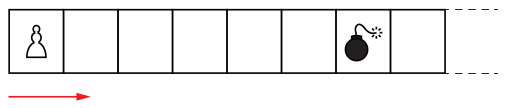
\includegraphics[scale=0.5]{imagens/unesp-2017.png}
			\end{center} Iniciada a jogada, a probabilidade de que o peão encerre a jogada na casa indicada na figura com a bomba é igual a:
			
			\begin{enumerate}[label=(\alph*), noitemsep]
				\item {37}/{324}
				\item {49}/{432}
				\item {23}/{144}
				\item {23}/{135}
				\item {23}/{216}
			\end{enumerate}

   \novaquestao{UFAM 2019}

            Considere a situação na qual as placas dos automóveis são formadas por duas letras seguidas de quatro algarismos. Numa determinada cidade, os carros só podem ser emplacados utilizando as letras P e Q e os algarismos ímpares, sem repetição de algarismos. Qual o número máximo de carros que podem ser emplacados nesta cidade?

                \begin{enumerate}[label=(\alph*), noitemsep]
	                \item 120.
	                \item 240.
	                \item 360.
	                \item 480.
	                \item 520.
                \end{enumerate}

            \novaquestao{UEA 2019}

            Para assistir a uma peça em determinado teatro, 5 amigos devem ocupar 5 poltronas posicionadas de forma consecutiva em uma mesma fileira. Aline, a única mulher do grupo, decidiu ocupar a poltrona do meio. Nesse caso, o número de maneiras diferentes que os 4 rapazes têm de se distribuírem nas poltronas restantes é 

                \begin{enumerate}[label=(\alph*), noitemsep]
	                \item 60.
	                \item 24.
	                \item 120.
	                \item 48.
	                \item 40.
                \end{enumerate}

            \novaquestao{UEA 2015}

            Por determinação do diretor, certa personagem de uma encenação folclórica deverá usar saia e blusa de cores diferentes em cada uma das suas 12 entradas em cena durante a apresentação. Desse modo, o número mínimo de peças (saias mais blusas) necessárias deverá ser igual a 

                \begin{enumerate}[label=(\alph*), noitemsep]
	                \item 12.
	                \item 6.
	                \item 9.
	                \item 7.
	                \item 8.
                \end{enumerate}

            \novaquestao{Enem 2022}

            Uma montadora de automóveis divulgou que oferta a seus clientes mais de 1 000 configurações diferentes de carro, variando o modelo, a motorização, os opcionais e a cor do veículo. Atualmente, ela oferece 7 modelos de carros com 2 tipos de motores: 1.0 e 1.6. Já em relação aos opcionais, existem 3 escolhas possíveis: central multimídia, rodas de liga leve e bancos de couro, podendo o cliente optar por incluir um, dois, três ou nenhum dos opcionais disponíveis.

            Para ser fiel à divulgação feita, a quantidade mínima de cores que a montadora deverá disponibilizar a seus clientes é

                \begin{enumerate}[label=(\alph*), noitemsep]
	                \item 8.
	                \item 9.
	                \item 11.
	                \item 18.
	                \item 24.
                \end{enumerate}

            \novaquestao{Enem 2012}

            O \textit{designer} português Miguel Neiva criou um sistema de símbolos que permite que pessoas daltônicas identifiquem cores.  O sistema consiste na utilização de símbolos que identificam as cores primárias (azul, amarelo e vermelho). Além disso, a justaposição de dois desses símbolos permite identificar cores secundárias (como o verde, que é o amarelo combinado com o azul). O preto e o branco são identificados por pequenos quadrados: o que simboliza o preto é cheio, enquanto o que simboliza o branco é vazio. Os símbolos que representam preto e branco também podem estar associados aos símbolos que identificam cores, significando se estas são claras ou escuras.
               
                \begin{flushright}
                \footnotesize
                \textbf{Folha de São Paulo.} Disponível em: \texttt{www1.folha.uol.com.br}. Acesso em: 18 fev. 2012 (adaptado).
                \end{flushright}

            De acordo com o texto, quantas cores podem ser representadas pelo sistema proposto?
            
                \begin{enumerate}[label=(\alph*), noitemsep]
	                \item 14.
	                \item 18.
	                \item 20.
	                \item 21.
	                \item 23.
                \end{enumerate}
		
		
	\end{multicols}
	
\end{document}
